\documentclass{standalone}
\usepackage{tikz}
\usetikzlibrary{patterns, positioning}
\usepackage[sfdefault]{ClearSans} %% option 'sfdefault' activates Clear Sans as the default text font
\usepackage[T1]{fontenc}

\begin{document}
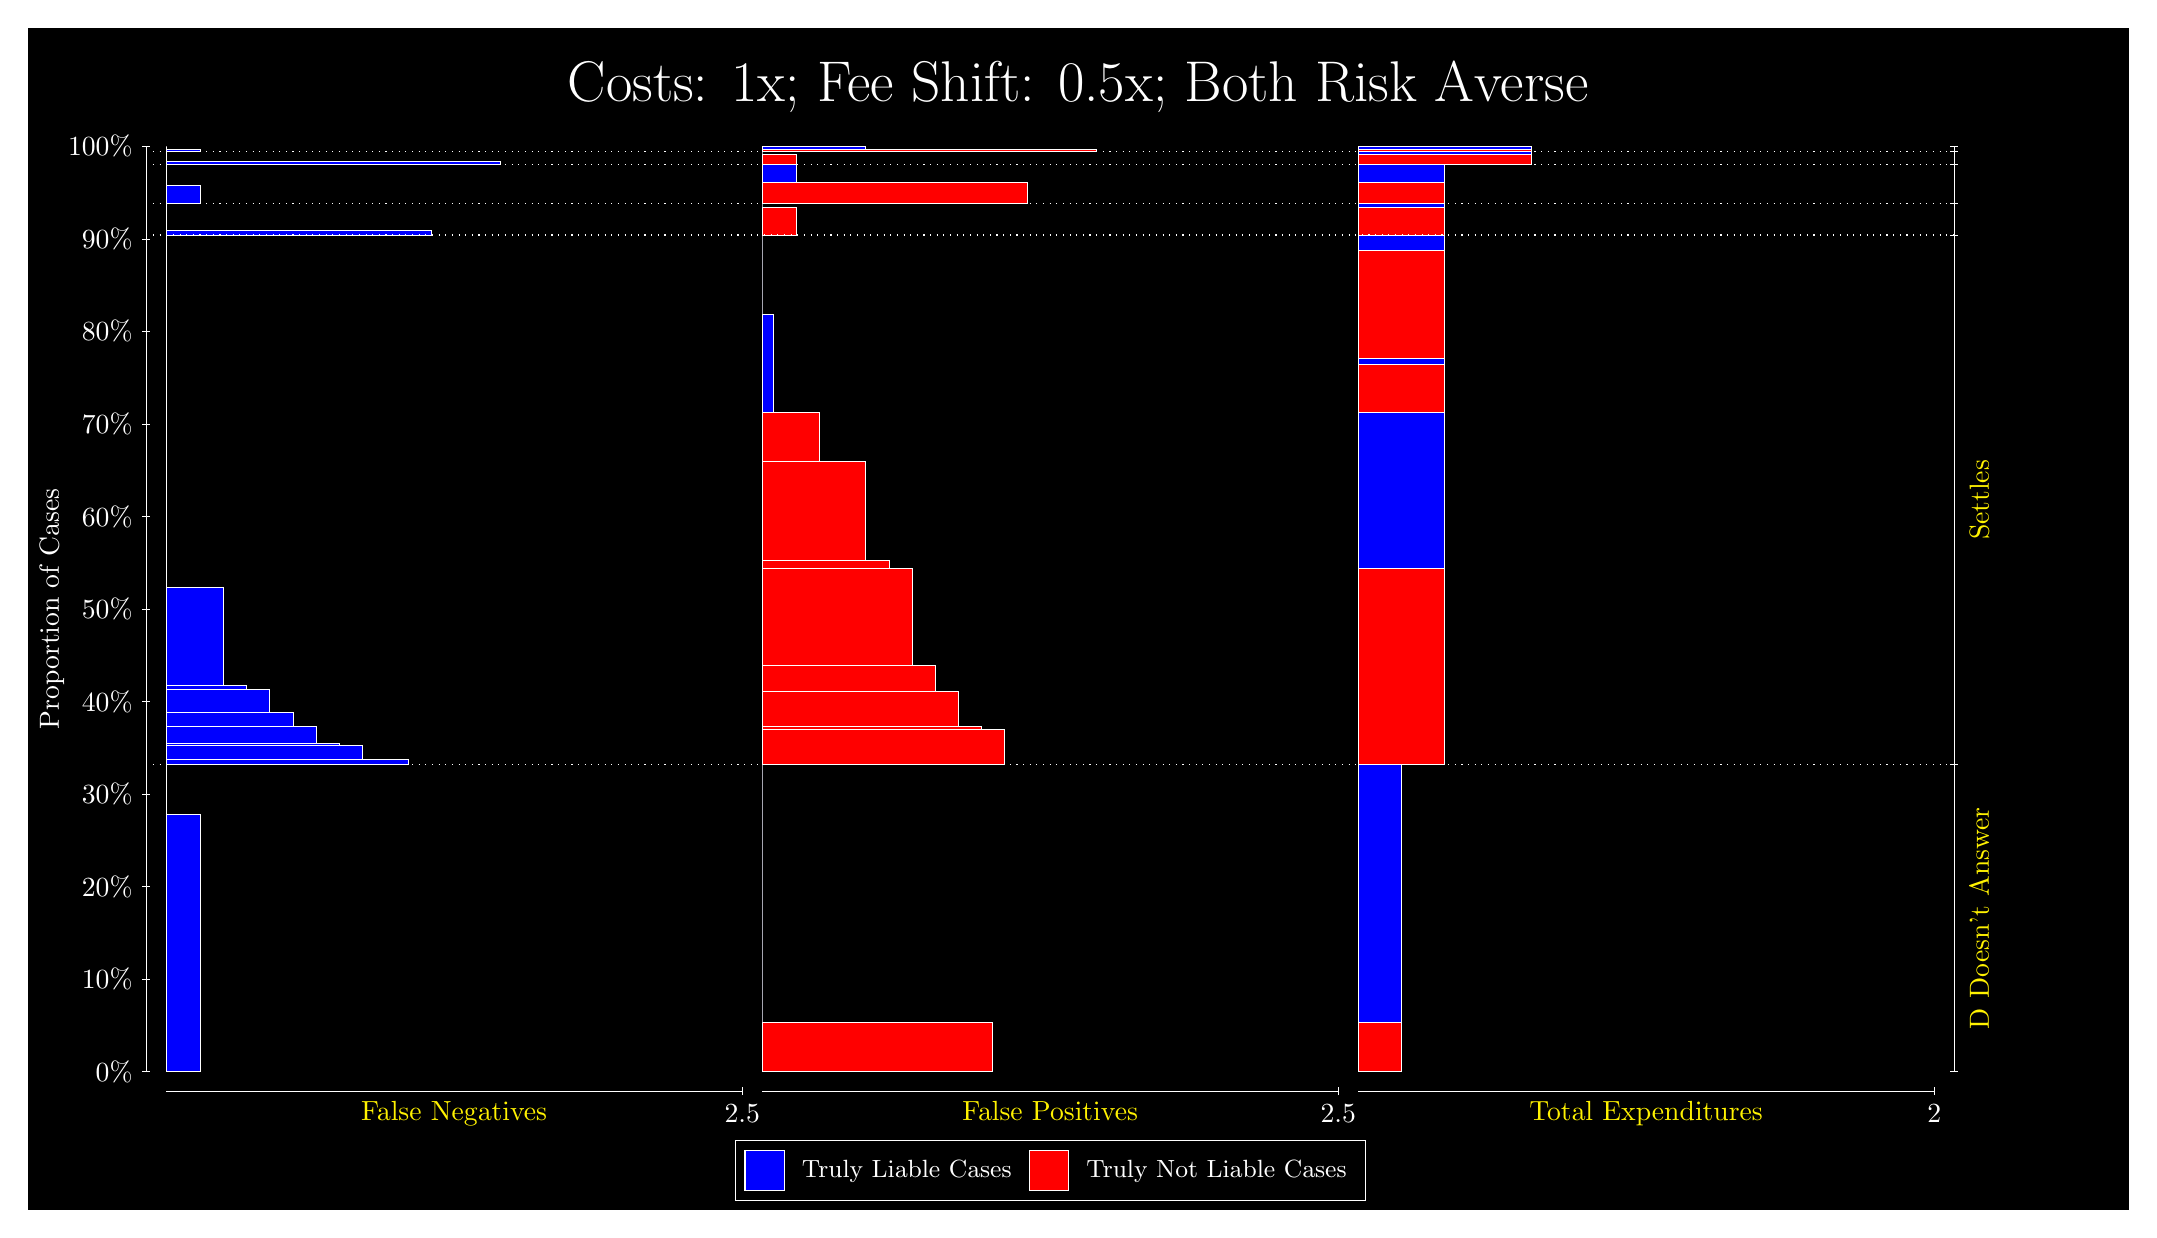
\begin{tikzpicture}
\draw[fill=black] (0,0) rectangle (26.667,15);
\draw[text=white] (0,13.5) rectangle (26.667,15) node[midway] {\huge Costs: 1x; Fee Shift: 0.5x; Both Risk Averse};
\draw[white, very thin] (1.5,1.75) -- (1.5,13.5);
\node[rotate=90, text=white, anchor=center] at (0.3, 7.625) {Proportion of Cases};
\draw[white, very thin] (1.45,1.75) -- (1.55,1.75);
\node[text=white, anchor=east] at (1.45, 1.75) {0\%};
\draw[white, very thin] (1.45,2.925) -- (1.55,2.925);
\node[text=white, anchor=east] at (1.45, 2.925) {10\%};
\draw[white, very thin] (1.45,4.1) -- (1.55,4.1);
\node[text=white, anchor=east] at (1.45, 4.1) {20\%};
\draw[white, very thin] (1.45,5.275) -- (1.55,5.275);
\node[text=white, anchor=east] at (1.45, 5.275) {30\%};
\draw[white, very thin] (1.45,6.45) -- (1.55,6.45);
\node[text=white, anchor=east] at (1.45, 6.45) {40\%};
\draw[white, very thin] (1.45,7.625) -- (1.55,7.625);
\node[text=white, anchor=east] at (1.45, 7.625) {50\%};
\draw[white, very thin] (1.45,8.8) -- (1.55,8.8);
\node[text=white, anchor=east] at (1.45, 8.8) {60\%};
\draw[white, very thin] (1.45,9.975) -- (1.55,9.975);
\node[text=white, anchor=east] at (1.45, 9.975) {70\%};
\draw[white, very thin] (1.45,11.15) -- (1.55,11.15);
\node[text=white, anchor=east] at (1.45, 11.15) {80\%};
\draw[white, very thin] (1.45,12.325) -- (1.55,12.325);
\node[text=white, anchor=east] at (1.45, 12.325) {90\%};
\draw[white, very thin] (1.45,13.5) -- (1.55,13.5);
\node[text=white, anchor=east] at (1.45, 13.5) {100\%};

\draw[white, very thin] (24.457,1.75) -- (24.457,13.5);
\draw[white, very thin] (24.407,1.75) -- (24.507,1.75);
\node[anchor=west] at (24.407, 1.75) {};
\draw[white, very thin] (24.407,5.6467) -- (24.507,5.6467);
\node[anchor=west] at (24.407, 5.6467) {};
\draw[white, very thin] (24.407,12.374) -- (24.507,12.374);
\node[anchor=west] at (24.407, 12.374) {};
\draw[white, very thin] (24.407,12.779) -- (24.507,12.779);
\node[anchor=west] at (24.407, 12.779) {};
\draw[white, very thin] (24.407,13.274) -- (24.507,13.274);
\node[anchor=west] at (24.407, 13.274) {};
\draw[white, very thin] (24.407,13.432) -- (24.507,13.432);
\node[anchor=west] at (24.407, 13.432) {};
\draw[white, very thin] (24.407,13.5) -- (24.507,13.5);
\node[anchor=west] at (24.407, 13.5) {};

\draw[white, very thin, fill=blue] (1.75,1.75) rectangle (2.1891,5.022);
\draw[white, very thin, fill=red] (1.75,5.022) rectangle (1.75,5.6467);
\draw[white, very thin, fill=blue] (1.75,5.6467) rectangle (4.8239,5.7158);
\draw[white, very thin, fill=blue] (1.75,5.7158) rectangle (4.2384,5.8983);
\draw[white, very thin, fill=blue] (1.75,5.8983) rectangle (3.9457,5.9142);
\draw[white, very thin, fill=blue] (1.75,5.9142) rectangle (3.6529,6.1364);
\draw[white, very thin, fill=blue] (1.75,6.1364) rectangle (3.3602,6.3126);
\draw[white, very thin, fill=blue] (1.75,6.3126) rectangle (3.0674,6.6109);
\draw[white, very thin, fill=blue] (1.75,6.6109) rectangle (2.7746,6.6535);
\draw[white, very thin, fill=blue] (1.75,6.6535) rectangle (2.4819,7.8974);
\draw[white, very thin, fill=red] (1.75,7.8974) rectangle (1.75,12.374);
\draw[white, very thin, fill=blue] (1.75,12.374) rectangle (5.1167,12.433);
\draw[white, very thin, fill=red] (1.75,12.433) rectangle (1.75,12.779);
\draw[white, very thin, fill=blue] (1.75,12.779) rectangle (2.1891,13.004);
\draw[white, very thin, fill=red] (1.75,13.004) rectangle (1.75,13.274);
\draw[white, very thin, fill=blue] (1.75,13.274) rectangle (5.9949,13.307);
\draw[white, very thin, fill=red] (1.75,13.307) rectangle (1.75,13.432);
\draw[white, very thin, fill=blue] (1.75,13.432) rectangle (2.1891,13.467);
\draw[white, very thin, fill=red] (1.75,13.467) rectangle (1.75,13.5);
\draw[white, very thin, fill=red] (9.3189,1.75) rectangle (12.246,2.3747);
\draw[white, very thin, fill=blue] (9.3189,2.3747) rectangle (9.3189,5.6467);
\draw[white, very thin, fill=red] (9.3189,5.6467) rectangle (12.393,6.0919);
\draw[white, very thin, fill=red] (9.3189,6.0919) rectangle (12.1,6.138);
\draw[white, very thin, fill=red] (9.3189,6.138) rectangle (11.807,6.5826);
\draw[white, very thin, fill=red] (9.3189,6.5826) rectangle (11.515,6.9111);
\draw[white, very thin, fill=red] (9.3189,6.9111) rectangle (11.222,8.1349);
\draw[white, very thin, fill=red] (9.3189,8.1349) rectangle (10.929,8.2378);
\draw[white, very thin, fill=red] (9.3189,8.2378) rectangle (10.636,9.503);
\draw[white, very thin, fill=red] (9.3189,9.503) rectangle (10.051,10.123);
\draw[white, very thin, fill=blue] (9.3189,10.123) rectangle (9.4652,11.367);
\draw[white, very thin, fill=blue] (9.3189,11.367) rectangle (9.3189,12.374);
\draw[white, very thin, fill=red] (9.3189,12.374) rectangle (9.758,12.72);
\draw[white, very thin, fill=blue] (9.3189,12.72) rectangle (9.3189,12.779);
\draw[white, very thin, fill=red] (9.3189,12.779) rectangle (12.686,13.049);
\draw[white, very thin, fill=blue] (9.3189,13.049) rectangle (9.758,13.274);
\draw[white, very thin, fill=red] (9.3189,13.274) rectangle (9.758,13.399);
\draw[white, very thin, fill=blue] (9.3189,13.399) rectangle (9.3189,13.432);
\draw[white, very thin, fill=red] (9.3189,13.432) rectangle (13.564,13.465);
\draw[white, very thin, fill=blue] (9.3189,13.465) rectangle (10.636,13.5);
\draw[white, very thin, fill=red] (16.888,1.75) rectangle (17.437,2.3747);
\draw[white, very thin, fill=blue] (16.888,2.3747) rectangle (17.437,5.6467);
\draw[white, very thin, fill=red] (16.888,5.6467) rectangle (17.986,8.1349);
\draw[white, very thin, fill=blue] (16.888,8.1349) rectangle (17.986,10.118);
\draw[white, very thin, fill=red] (16.888,10.118) rectangle (17.986,10.738);
\draw[white, very thin, fill=blue] (16.888,10.738) rectangle (17.986,10.808);
\draw[white, very thin, fill=red] (16.888,10.808) rectangle (17.986,12.176);
\draw[white, very thin, fill=blue] (16.888,12.176) rectangle (17.986,12.374);
\draw[white, very thin, fill=red] (16.888,12.374) rectangle (17.986,12.72);
\draw[white, very thin, fill=blue] (16.888,12.72) rectangle (17.986,12.779);
\draw[white, very thin, fill=red] (16.888,12.779) rectangle (17.986,13.049);
\draw[white, very thin, fill=blue] (16.888,13.049) rectangle (17.986,13.274);
\draw[white, very thin, fill=red] (16.888,13.274) rectangle (19.083,13.399);
\draw[white, very thin, fill=blue] (16.888,13.399) rectangle (19.083,13.432);
\draw[white, very thin, fill=red] (16.888,13.432) rectangle (19.083,13.465);
\draw[white, very thin, fill=blue] (16.888,13.465) rectangle (19.083,13.5);
\draw[white, dotted] (1.5,5.6467) -- (24.457,5.6467);
\draw[white, dotted] (1.5,12.374) -- (24.457,12.374);
\draw[white, dotted] (1.5,12.779) -- (24.457,12.779);
\draw[white, dotted] (1.5,13.274) -- (24.457,13.274);
\draw[white, dotted] (1.5,13.432) -- (24.457,13.432);
\draw[white, very thin] (1.75,1.5) -- (9.0689,1.5);
\node[text=yellow, anchor=north] at (5.4094, 1.5) {False Negatives};
\draw[white, very thin] (9.0689,1.45) -- (9.0689,1.55);
\node[text=white, anchor=north] at (9.0689, 1.45) {2.5};

\draw[white, very thin] (9.3189,1.5) -- (16.638,1.5);
\node[text=yellow, anchor=north] at (12.978, 1.5) {False Positives};
\draw[white, very thin] (16.638,1.45) -- (16.638,1.55);
\node[text=white, anchor=north] at (16.638, 1.45) {2.5};

\draw[white, very thin] (16.888,1.5) -- (24.207,1.5);
\node[text=yellow, anchor=north] at (20.547, 1.5) {Total Expenditures};
\draw[white, very thin] (24.207,1.45) -- (24.207,1.55);
\node[text=white, anchor=north] at (24.207, 1.45) {2};

\node[text=yellow, centered, rotate=90] at (24.777, 3.6984) {D Doesn't Answer};
\node[text=yellow, centered, rotate=90] at (24.777, 9.0103) {Settles};





\draw (12.978300999999998,1.5) node[draw=none] (baseCoordinate) {};
\begin{scope}[align=center]
        \matrix[scale=0.5, draw=white, below=0.5cm of baseCoordinate, nodes={draw}, column sep=0.1cm]{
            \node[rectangle, draw, minimum width=0.5cm, minimum height=0.5cm, fill=blue] {}; &
            \node[draw=none, font=\small, text=white] (B) {Truly Liable Cases}; &
            \node[rectangle, draw, minimum width=0.5cm, minimum height=0.5cm, fill=red] {}; &
            \node[draw=none, font=\small, text=white] (B) {Truly Not Liable Cases}; \\
            };
\end{scope}

\end{tikzpicture}
\end{document}